\documentclass[parskip=half, fontsize=12pt]{scrartcl}
\usepackage{float} % Enables exact-placement of figures
\usepackage[hidelinks]{hyperref} % Enables linking
\usepackage[margin=1in]{geometry}
\usepackage{graphicx}
\usepackage{mathptmx} % Adds Times New Roman
\usepackage{longtable}
\usepackage{makecell}
\usepackage{setspace}

\graphicspath{ {./images/} }
\setstretch{1.2} % From setspace package

\fontfamily{ptm}\selectfont

\title{OurSPIM}
\subtitle{Browser-Based MIPS64 Emulator}
\author{
    Kevin Cahalan
    \and
    Jerrett Longworth
    \and
    Huy Nguyen
    \and
    Evan Raiford
    \and
    Jimmie Smith
}

\begin{document}
\renewcommand*{\titlepagestyle}{empty}
\maketitle
\clearpage

\pagenumbering{roman}
\setcounter{page}{1}
\tableofcontents
\clearpage


\pagenumbering{arabic}
\setcounter{page}{1}
\section{Executive Summary}

At some point when learning computer science, students have to learn about assembly languages and instruction set architectures and, in most universities, the assembly language of choice is MIPS32. If students proceed to take more advanced courses centered on computer architecture, they inevitably encounter MIPS64 in that process, as well. While there are various emulators and tools available for students and instructors to use to learn and teach MIPS, they almost always have some issue holding them back from being the best tools they can be. Some of them have obtuse interfaces, others have not been updated in years or decades making running them on modern hardware difficult, and almost all of them only support MIPS32 and so cannot be used in learning MIPS64. Because of this, learning low-level programming concepts, a task that already is difficult in and of itself, is even tougher for most students than it needs to be.

Our solution to this issue is OurSPIM. OurSPIM is a MIPS emulator that supports both MIPS32 and MIPS64 and runs within a browser. In OurSPIM, people will be able to write and run MIPS32 and MIPS64 programs in browser with an enhanced text editor that will feature step-through debugging, the ability to view register contents, and recognition of MIPS pseudo-instructions in a modern looking, easy to use interface. Making an emulator that supports both major versions of MIPS means that students will be able to use OurSPIM throughout a large part of their low-level programming education. Being browser based, the barrier for entry is much lower than downloaded software and people will be able to access a MIPS emulator from anywhere. Having modern features like step-through debugging and register viewing will make the development experience more similar to modern languages and easier to work with.

As mentioned previously, OurSPIM will be a browser-based system. The code for the project will be written primarily in Rust so we can take advantage of its memory management systems and we will use JavaScript where necessary. For the text editing interface, we will use Monaco. The backend of OurSPIM will be minimal with none of the processing work happening there; it will exist only to serve the frontend to the user. In the backend, we will be using Docker as a container for the Rust code. OurSPIM will implement almost all available instructions within MIPS32 and MIPS64 with the exception of a few instructions that are needed only for interacting with operating systems.

The main goal of the OurSPIM project is to make a system that facilitates learning MIPS ISAs and low level programming concepts. To that end, we are planning on making OurSPIM available to use by anyone at no cost. Similarly, we are planning to put OurSPIM under the GNU General Public License to allow anybody to view the code that we have written and modify it as they see fit and then distribute it to others freely. 


\section{Project Description}
The current options for MIPS emulation software, we feel, are overly-complex or use out-of-date frameworks. Our project aims to be a new, alternative MIPS emulation software that is easier to digest compared to existing options. Ideally, starting a simulation of a MIPS processor should be as easy as opening a Replit project, and there should be minimal resistance for a newcomer to learn MIPS. The current go-to option for educational MIPS simulation is SPIM. While it has a rich feature-set, SPIM is no longer actively maintained, is aging since its original release in 1990, and is not user-friendly by modern standards. Additionally, SPIM only supports MIPS32, meaning the 64-bit extension of MIPS, MIPS64, is unsupported. Many students do not attempt to use SPIM unless required by their courses due to these limitations, and our goal is to change this scenario with our alternative. Students should be interested and want to use the simulator to study for classes and self-taught individuals should be able to use it to satisfy curiosity. Both groups of people should experience a minimal learning curve when it comes to interacting with the MIPS pipeline.

Our solution for a simulator of minimal learning resistance is ``OurSPIM,'' named as such to reflect students of our time. Technology has progressed past dial-up networking, for example, and the web has become the largest source for information in history. The hope is for OurSPIM to become the standard for MIPS education, as a standard emulator for both MIPS32 and MIPS64. Every professor and course instructor should recommend OurSPIM.

Many similar variations of this project currently already exist online, however these variations are missing features that we believe are important. Most critically almost none of the options out there support MIPS64. While OurSPIM may not be the perfect solution for teaching assembly, our project aims to make, or at least contribute to making, MIPS less complex for beginners to learn, online.


\section{Broader Impacts}
The end goal of this project is to help make it easier for people to learn about the MIPS instruction set architecture and hopefully create an intuitive and visually pleasing system with which people can interact with MIPS32 and MIPS64. This project aims to lower some of the barriers that people commonly struggle with when trying to learn about computer architecture and low-level programming. This way, OurSPIM could help redefine how MIPS simulation is used in education, as learning MIPS would become more accessible. Since the project will be built entirely to run in a web browser, it is not only more accessible for students at UCF, but for learners all over the world.

Additionally, with the project being available online, and thus immediately accessible by any computer with a modern web browser, OurSPIM would be a great option for professors and course instructors to use during lectures, as they do not have to spend time or effort to install additional software to use in classroom computers. In this way, OurSPIM could become the de facto way of teaching MIPS. By making MIPS easier to teach within lectures and easier for students to use on their own, we aim to make low-level programming concepts overall easier for students to learn.



\section{Project Function}
\begin{itemize}
    \item MIPS32 support
    \item MIPS64 Support
    \item Step-through debugging
    \item Register value view
    \item Reverse execution
    \item Mouse hover instruction assistance
    \item Homemade parser to recognize alternatives to pseudo-MIPS instructions
    \item Possible display window for graphics
\end{itemize}


\section{Legal, Ethical, and Privacy Issues}
We do not foresee any privacy issues based on our needs. The MIPS simulation will run on the front-end of the website and our base design does not make use of accounts for users so there is nothing that is stored on the backend. Since we are not storing any user information, there should not be any privacy issues.

Similarly, we do not foresee any ethical issues. We are not planning on trying to monetize what we are trying to build nor is it gathering data on people. What we are hoping to build is purely an educational tool so we do not see the possibility of having any ethical issues with OurSPIM.

We are currently hoping to put the OurSPIM project under the GNU General Public License. Our hope is to make OurSPIM available freely for anybody to use and for them to be able to take what we have built and then modify it to fit their needs, as well. The GPL aligns with that exactly. 

Putting the OurSPIM project under the GNU General Public License would also ensure that we do not have to worry about any issues with the copyright of the software that we build. Since the GPL uses the idea of copyleft to make it so that anybody is allowed to use, distribute, and modify so that is useful in what ways they see fit. Plainly, we should not run into any issues stemming from copyright because we are only taking advantage of the copyright on the software to the extent that it allows everybody free access to it.

The areas that we may run into legal issues is with the software that already exists that we are basing our software off of and the companies whose architectures we are seeking to simulate. The idea for our software is based on what the MIPS simulator, SPIM, has already done which is immediately apparent with our name, OurSPIM. As such, one thing we will be doing in the first semester is having discussions about the legality of basing our name so directly on the works of an unaffiliated group and whether or not we might need to change our name to something different. The other issue on this front stems from the fact that we are very specifically trying to build software that will simulate the architectures created by MIPS Technologies. As such, we will need to research and make sure that we will not run into any issues from them because of that. Since what we are building is not for profit and is purely a tool for education and there have been teams before that have built similar tools, such as SPIM, we do not foresee this being a legal issue.


\section{Financing}
OurSPIM is a project that was pitched by a student, so funding support from a sponsor is not available to our group. However with the planned scope of this project, we foresee that major funding will not be necessary, as it will run entirely client-side in a web browser, and needs no paid components to be developed. At this time, the only likely cost associated with OurSPIM would be for server hosting and deployment, but many options for this have free tiers available. For example, Heroku currently offers free dynamic hosting for projects up to 1,000 hours, however this option was immediately tossed since Heroku will be dropping their free tier in November 2022, as OurSPIM will continue to be developed well into Spring 2023. Other free hosting options currently being considered include UCF's Linux server, Eustis3, or GitHub Pages via GitHub Actions. However, we are hoping that what we build will be useful after we graduate and so want to ensure it is still available after we have all left UCF so we are steering away from Eustis3 as an option. A paid alternative may be to have all members pitch in a nominal amount of money to rent a Linux VPS server during the duration of the project to deploy on. Financing is not an issue.


\section{Goals}
\begin{itemize}
    \item To be able to deliver a stable version of this project by the last due date:
    \begin{itemize}
        \item Complete Frontend UI and core logic
        \item Will be able to showcase
    \end{itemize}
    \item To learn new technologies and be flexible
    \item To gain work experience
    \item To gain teamwork and time management skills
    \item To gain a more intimate knowledge of how a simulator of something such as MIPS functions 
\end{itemize}



\section{Objectives}
\begin{itemize}
    \item Build a fully functioning website that has all of the features of our minimum viable product and as many of the extra features as we are able to get in.
    \begin{itemize}
        \item Have weekly meetings with our team to ensure we are all on the same page on progress and so any issues we are facing can be taken care of to the best of all of our abilities, collectively.
        \item Work on the project and the design document multiple times throughout each week to guarantee frequent and consistent progress is made toward our milestones.
        \item Meet the deadlines for all of our project milestones.
    \end{itemize}

    \item Research the technologies that will best suit the project that we are trying to make.
    \begin{itemize}
        \item Review the design documents for both MIPS32 and MIPS64 to make sure that we are able to build a project that implements both Instruction Set Architectures to the best of our abilities
        \item Review how the existing SPIM software functions
        \item Learn how the Rust Programming Language functions
    \end{itemize}
    
    \item Structure our work so we are able to adhere to best practices for software engineering
    \begin{itemize}
        \item Build and stick to a detailed but flexible Gantt Chart
        \item Use GitHub as version control in case we need to revert to a previous stable build
        \item Write Unit Tests as we work so that we can make sure any new additions to our build do not break any features that were already implemented
    \end{itemize}
\end{itemize}



\section{Project Motivation}
The motivations for this project come from many different directions; mainly awesomeness, personal educational benefits, clear direction, and job interviews. There is just something awesome about writing an emulator. It's like magic to see software run in a simulation. Currently there's a solid demand out there in the cyber industry for custom emulation. In the cyber world hacking has been becoming harder and harder. Everyone is trying to automate. In part with AI, in part with special algorithms and software. For much of the automation there's a need for scale and state access. The ability to know everything, ram, flash, register states, and so on, is very important. With real hardware your access to know exactly what the system is doing is limited. Real hardware can also be very costly, on the order of millions per unit. Sometimes real hardware can be unassable by normal means, for example weapon systems. Security researchers want to be able to make as many virtual environments as possible with minimal cost. They want to be able to understand anything that a system is doing. To become a professional emulator developer, small steps of learning are required. By writing OurSpim our team will be taking a small step, we should all leave with a better understanding of the world of emulation development.



\section{Individual Motivations}
\subsection{Kevin Cahalan}
\begin{figure}[H]
    \centering
    
\includegraphics[height=7cm]{profile-kevin}
\end{figure}

For a while I have been wanting to write an awesome emulator. Things kept getting in the way, I never got to it. Ever since I first started learning python, I have had an urge to get the ultimate understanding of computers. Python sucked, it did not feel like programming. Writing Python felt like telling a program what to do, not a computer. There was clearly magic undernither. I hated having these magical devices out there that I could simply not fathom or imagine. Computers seemed to be true magic. To go further down my journey of getting a true understanding of computers, I started learning C. C was a breath of free air. The more I programmed in C, the more computers made sense. Writing my first emulator, some emulator for a computer from the 70s, I took a big step in learning the magic behind computing. Emulation development turns out to be a great way for clearing away the magic property of computers. When writing an emulator, you're effectively writing your own computer in software. By working on OurSPIM I will be continuing my journey to get the ultimate understanding of computation. I will further fight the mysterious magic of computation.

Another big individual motivation for this are the job prospects. There's solid money out there for emulation development. Emulators have all sorts of uses, hacking, training, testing, legacy hardware replacement, and so on. In the world of professional hacking, the need for automation fits hand in hand with emulator development. Automated bug finders need a surface to play with. Preferably a scalable surface. Using real hardware can get super expensive very fast. It can be millions or billions of dollars, sometimes impossible to get. With training it is not best to trust a new person with expensive equipment. Issues of money and safety come into play. It would not be the best idea to just drop someone into an f-35, you start them with an accurate flight simulator. So accurate that you emulate the computers within the aircraft for the simulation. When testing new software for an f-35, initially using a real aircraft would be unsafe. You test your software in emulation. In the world of banking there are old legacy computers that need to be replaced. Re-writing the software for these ancient computers can be very risky and costly. The solution is to write an emulation layer to port so that the old software could run on modern computers. With many more examples out there, emulation happens to be very important for this world. And the best part of all this, there's big money in the industry.


\subsection{Jerrett Longworth}
\begin{figure}[H]
    \centering
    
\includegraphics[height=7cm]{profile-jerrett}
\end{figure}

From first being introduced to computer architecture and processor logic and design at UCF, I was immediately interested in the subject area and wanted to learn more. This topic, along with similar low-level topics such as assembly languages, became a focus of mine throughout my Computer Science studies. In the popular open-world sandbox game Minecraft, I designed logic and built circuitry from scratch for a system that takes a binary number and displays it on an in-game seven-segment display. While studying Computer Logic and Organization (CDA 3103) with Sarah Angell, I had already begun to think about the utility and overall interest factor of having a live graphical representation of a CPU performing instructions in its pipeline, not only for an Instruction Set Architecture like MIPS, but for x86 and ARM as well. OurSPIM can offer this first step into creating a visualization such as this.

I have thought about various forms, both in hardware and software, that could achieve this effect. Inspired by an engineering sample of an Nvidia 30-series graphics card, a hardware approach could have a dedicated pin on the processor that reports some basic information like the current instruction opcode or instruction pointer. A software approach could be a graphical overlay over a high-definition image of the internals of a CPU. A user could be given a live view of the bits changing as a virtual CPU executes instructions, and you could pan and zoom around the parts of the processor to see values located in registers, memory, and other components.

Based on these ideas, I feel OurSPIM is an incredibly valuable project, both for the educational factor for classes like CDA 3103, but also for the personal enjoyment and satisfaction of watching this piece of technology run at its most exposed state.

Another reason why this project is important to me is due to my affiliation with Wiki Knights, which is a student organization dedicated to reducing or eliminating the costs of textbooks and homework access codes by encouraging the adoption of Open Educational Resources (OER) in courses across the university. This group has already been developing a free Introduction to C Programming (COP 3223) textbook with examples and practice problems, which is currently deployed in classes as of the time of writing. Further development is active within the group to re-open the Adaptive Learning Engine project authored by the ALOSI Labs as a collaboration between Harvard University's Office of the Vice Provost for Advances in Learning and Microsoft. Along these efforts, an open-source project such as OurSPIM offers another free resource for students, course instructors, and researchers in areas related to computer architecture.


\subsection{Jimmie Smith}
\begin{figure}[H]
    \centering
    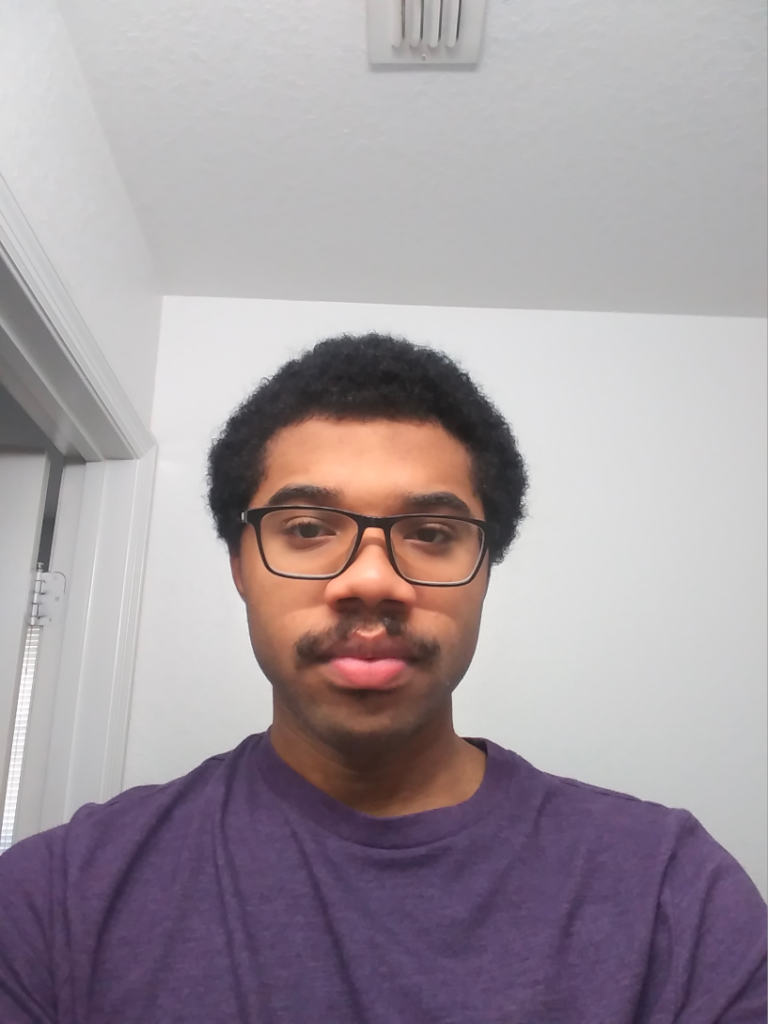
\includegraphics[height=7cm]{profile-jimmie}
\end{figure}

While I pitched a project for this class with a similar topic, I figured this was a more noble project to do. As someone who enjoyed CDA3103 and EEL4768, OurSPIM could be the first step to educating people who are interested in Assembly in a friendlier environment. Funnily enough, my pitch has the same underlying goal as OurSPIM of modernizing the ``old'' workflow with enhancements and visual feedback that makes it easier for the user to understand the concept and have fun with it, too. Recently, I've been learning about the Motorola 68000 since it was a CPU that was used extensively back then, so I have a general feel for CISC and RISC assembly with their concepts. I also have an affinity for emulation since it is pretty fun to explore older systems, and you can preserve them, study them, and make new tools for them.

This is my first time being relegated to front-end development solely so it is a huge responsibility to make sure the whole suite is presented in an appropriate manner. Even though I have been assigned to work on the frontend with Rust, I am excited to understand Rust since I heard people giving praise for its design compared to C. I have a few ideas of my own on how I want the program to look since user experience is key. Learning Assembly is hard to sell compared to high-level languages, there are not that many good online tutorials for assembly, it's much more verbose, and it has a steeper learning curve so interactivity is my top-priority. This is a nice challenge for me since I have to constantly ask myself how to make OurSPIM fun to use while the backend focuses on creating a good emulation core.

My experience with MIPS in the past was easy-going at first, but by the time I took Computer Architecture it became overwhelming especially when it came to the different datapaths. By the end of the course, I was having a difficult time understanding the concepts and how significant they are. I had a harder time finding any tools that would help me understand MIPS64 compared to MIPS32, so OurSPIM would fill in that gap. With OurSPIM, it would not only remedy any confusions with MIPS64's concepts but it can also be the basis for studying different types of architecture and their featureset.


\subsection{Evan Raiford}
\begin{figure}[H]
    \centering
    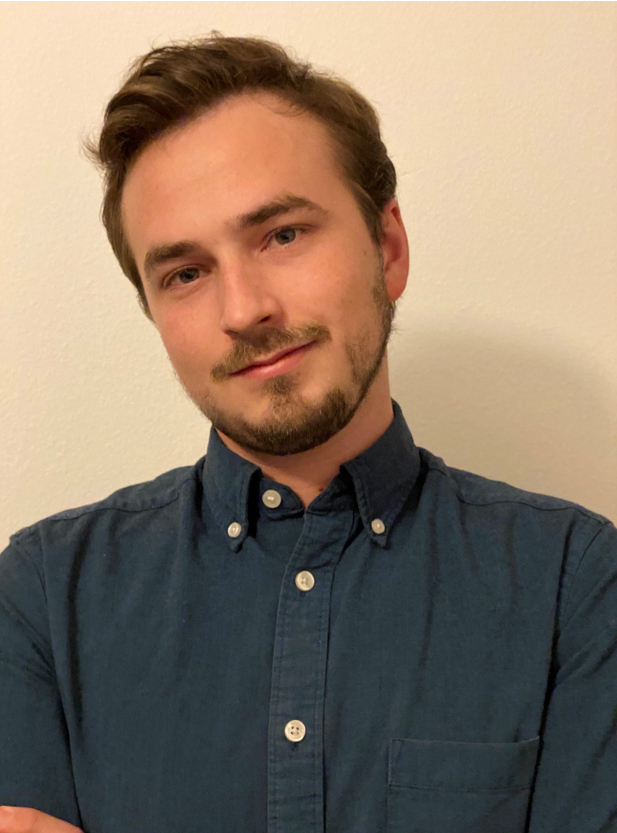
\includegraphics[height=7cm]{profile-evan}
\end{figure}

My motivation for this project stems from multiple different places. The first reason is that I see a need for the existence of a tool such as this. One of the restricted electives I chose to take was EEL4768, Computer Architecture, and a large part of that class was understanding the changes necessary to implement a 64-bit system as opposed to a 32-bit system and the language used to detail these changes was MIPS64. Examples drawn out on the board and thorough explanations are great tools to assist in learning but for many people, myself included, the best way to get a grasp on things is to try them out themselves. Having a version of MIPS64 readily accessible would be a great tool to help students learn.

A second, albeit related, reason I am motivated for this project is that I am hopeful that we can build a tool that makes MIPS more approachable for students. One of my absolute favorite things about my experience earning my computer science degree has been building a solid understanding of how a computer works from the bottom up. Assembly languages, such as MIPS, are one of the foundational aspects of this. However, assembly languages can often come across as intimidating and hard to approach for new learners so students frequently only learn enough to get through their class. I think a solid understanding of basic instruction set architectures is vital to being a well-rounded software developer. My hope is that the OurSPIM project will help make MIPS and low-level programming concepts more approachable for the average student.

The idea of making OurSPIM browser based is another reason I am motivated for this project. Making it browser-based makes the software more approachable for students since they would not need to download anything onto their devices to use it. It also means it is more readily accessible for instructors. If an instructor wants to use software that has to be downloaded in a lecture hall, they often do not have the option to download the software onto whatever device is used in the lecture hall so they, instead, have to bring their own device with them and hook that up to the projector in order to use the software in a lecture. Having OurSPIM online circumvents that issue entirely. If somebody wanted to use OurSPIM in a lecture, the software is accessible through the browser so all they would need to do is navigate to the website.

Another reason that I am motivated for this project is the lack of a sponsor. Having a sponsor on a project does give a lot of benefits like financial backing, industry experience and advice, and a guiding hand. However, they often also come with their own motivations for the project, often hoping to use the tool to help bolster their business. Doing a project without a bespoke sponsor ensures that whatever we make is not beholden to somebody else's vision of what it can or should be. Doing it without a sponsor also ensures that our end product is one made wholly by us. Any issues we have along the way, we ourselves are the ones that overcome them. The project that we make is one that we are able to make solely on the experience that we have gained ourselves either on our own or at UCF.


\subsection{Huy Nguyen}
\begin{figure}[H]
    \centering
    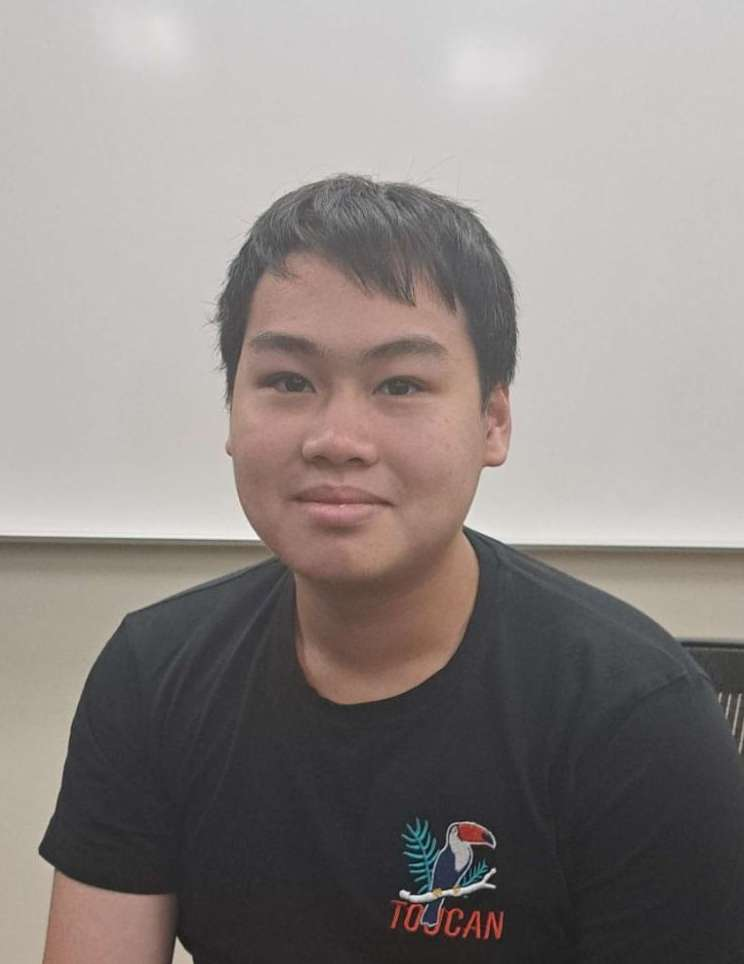
\includegraphics[height=7cm]{profile-huy}
\end{figure}

My motivation for the project stems from my experience with some of the materials needed for this project, about the MIPS pipeline. The idea of an accessible web-based MIPS emulation would have helped me and my peers a lot back when I was studying Computer Architecture and System Softwares. It would also make these subjects a lot easier on students who need to take those, as well as being interested to learn more about MIPS, which in turn would help with easier and more understandable teaching than what me and my peers went through during those classes in the past.

I am also attracted to this project by the prospect of not needing a sponsor. Not having a sponsor means a few things. One of those things is that we as a group are not constrained by the sponsors' demands, which means we can be more comfortable in giving project ideas so that it looks like what the group thinks it is, not what anyone outside thinks it is. This would also mean anything we need to spend on for the project we have to spend ourselves, and we also have to set deadlines ourselves, which may be hard or distracting. However, I believe this will get me more familiar with these kinds of projects where the idea is from a single person and it is up to me and my group to expand on, not just a pre-laid road by a company. Although I may lose the experience of working with a sponsor, I currently have an opportunity to make a project that I may be able to talk about in the future, which is this project. This project would also hopefully improve my skills working with my teammates, as it will undoubtedly help with further group projects and careers in general in the future.

This project also seems like an opportunity to come in contact with more variety in coding, as the project currently aims to run mostly on the frontend in Rust, a language I have never touched before. After having a look at it, it seems solid, so it made me look forward to using it on a project and adding one more language to my arsenal. That will also mean I get to learn more about web development, specifically running a simulator online, about what it entails.



\section{Project Requirements and Specifications}
This project is going to have two main sections: the non-graphical frontend, and the graphical frontend.  The initial plan for the server is that it will be very bare bones. There will be minimal API calls; it just needs to deploy the frontend. With the server being very minimal, the frontend will be very fancy and will be the center of the project. In a way, OurSPIM is very similar to a desktop application.

The non-graphical frontend is where the meat of the project is going to sit, most importantly the emulation core. This core is going to be initially written in a simplistic way both emulating a CPU and an operating system. It should end up supporting almost all 32 and 64 bit MIPS instructions. There are some instructions for stuff such as messing with paging and virtual- physical mappings; these instructions should be implemented as part of a stretch goal. Such instructions are only really needed for operating system development. Obviously, supporting these instructions would be awesome, but the main goal of being an emulator to teach MIPS must come first. 

Along with the emulation core, there needs to be a way to make instructions to execute. It is not acceptable to expect the user to upload a memory layout with already assembled instructions. Somehow, user written instructions need to be converted in binary format. There needs to be an association between ascii instructions and binary in memory. This is where parsing and assembling come in. There are many different options for approaching this problem. It's possible to write a custom assembler and parser, and there are many benefits to this. Alternatively, it might also be possible to post an existing assembler to the web.

An important piece to this project is a nice graphical frontend. One of the main issues out there with existing emulators is that they all have old fishy frontends. OurSPIM should be modern and familiar. A user should feel at home when using this emulator, like how someone using Firefox would feel when using Chrome. Our interface should be similar to that of Visual Studio Code, Repl.it, or GodBolt. The key to this familiarity is either base our frontend on the Monaco or CodeMirror libraries. 



\section{Group Member Ideas}
\subsection{Kevin Calahan}
\begin{itemize}
    \item The project itself
    \item The use of Rust for programming both the backend and frontend
\end{itemize}


\subsection{Jerrett Longworth}
\begin{itemize}
    \item Interactive live view of the emulator pipeline with access to memory and register contents. A user could hover over various components or traces with their mouse to see their current contents.
    \item Alternative live view of the pipeline, which is overlaid onto a real-world image of a CPU die. This could be zoomed or panned to see individual bits in any of the components.
    \item Ability to view and change memory and register contents during execution.
    \item Communication to and from the user with a virtual display and input, communicated through an emulated bus.
    \item A ``tutorial/educator mode,'' which would allow an educator to create overlays and control the interface automatically to guide students to learn about a specific concept.
    \item A ``quiz mode,'' which would allow an educator to create overlays similar to the ``tutorial mode,'' but with interactive questions and problems that can report results to an LMS such as Instructure Canvas.
\end{itemize}


\subsection{Jimmie Smith}
\begin{itemize}
    \item As a design goal, OurSPIM should not only support MIPS64 but it should be designed openly to load in different emulators of CPUs and their respective datapaths (if available). This would require some careful planning, but should be feasible since this is being built from scratch.
    \item Having a live debugger for OurSPIM would be a simple feature to implement, but could streamline the debugging process even more. 
    \item Since this is a web application, I think having customizable options would elevate the user experience like dark mode, color-coding for instructions, registers, etc. 
\end{itemize}


\subsection{Evan Raiford}
\begin{itemize}
    \item An account system so that users are able to store something that they have been working on and then come back and continue working on it later. This would also allow lecturers the opportunity to store work that they can then access in a lecture.
    \item A tool that explains the function of instructions
    \item Prefabricated programs that users can take a look at and mess around with to get a feel for how things are done in MIPS. A brief overview and explanation of what is being done and why could accompany it 
\end{itemize}


\subsection{Huy Nguyen}
\begin{itemize}
    \item We can make the frontend look more accessible by giving the MIPS pipeline map more space as well as making the UI fit viewing mode, or hide them.
    \item Testing on Eustis3. Although I do think that this may not work or take forever to load the frontend since our project is frontend heavy.
    \item Admin accounts for testing frontends and account creations if necessary
\end{itemize}



\section{Use Case Diagrams}
\begin{figure}[H]
    \centering
    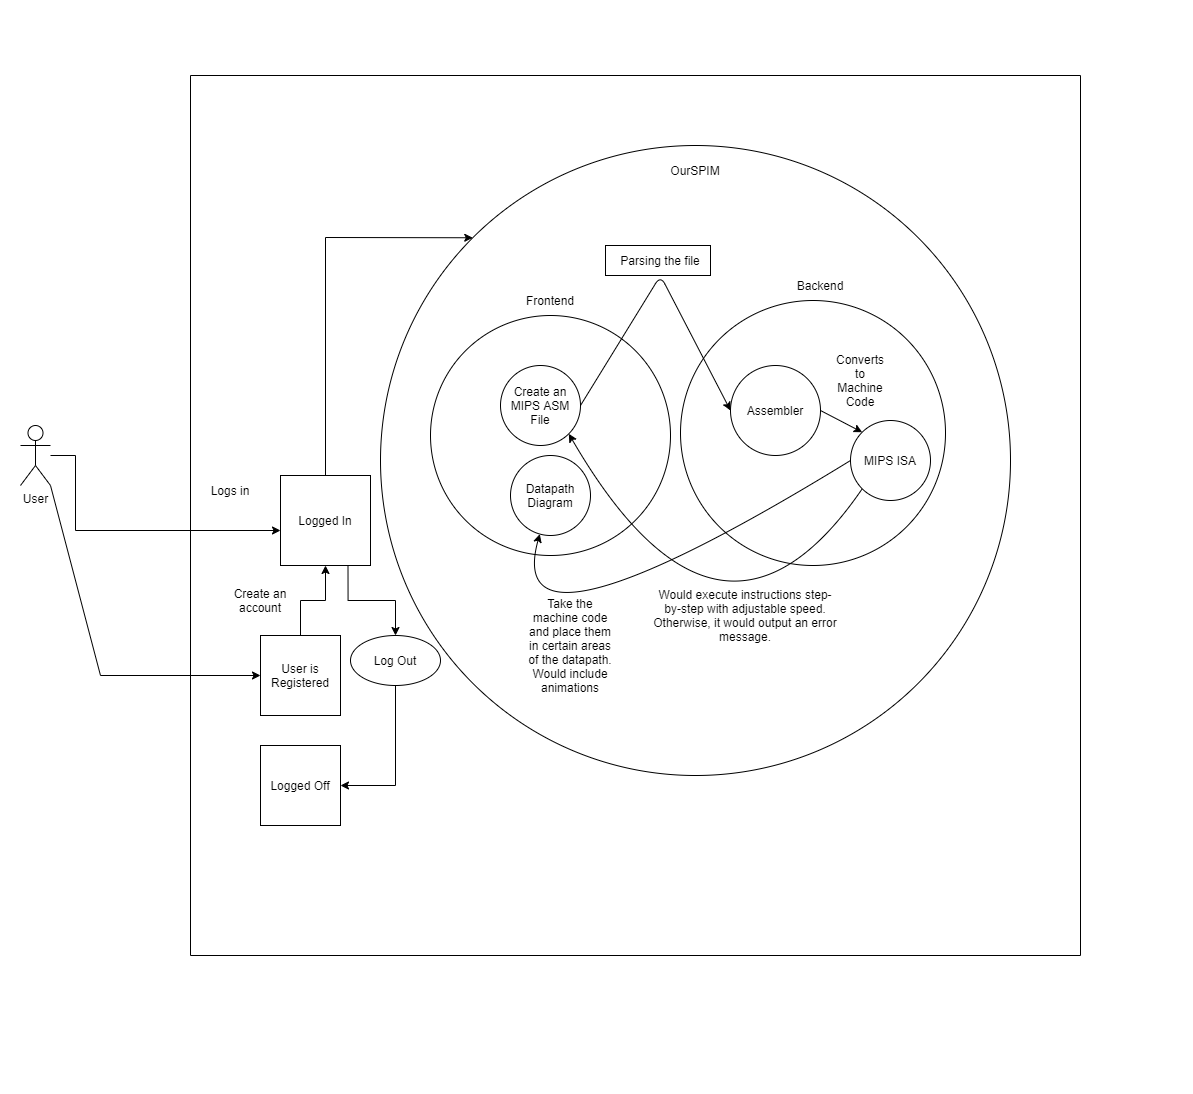
\includegraphics[width=\textwidth]{use-case-diagram}
    \caption{Use Case Diagram of OurSPIM}
\end{figure}



\section{Block Diagrams}
\begin{figure}[H]
    \centering
    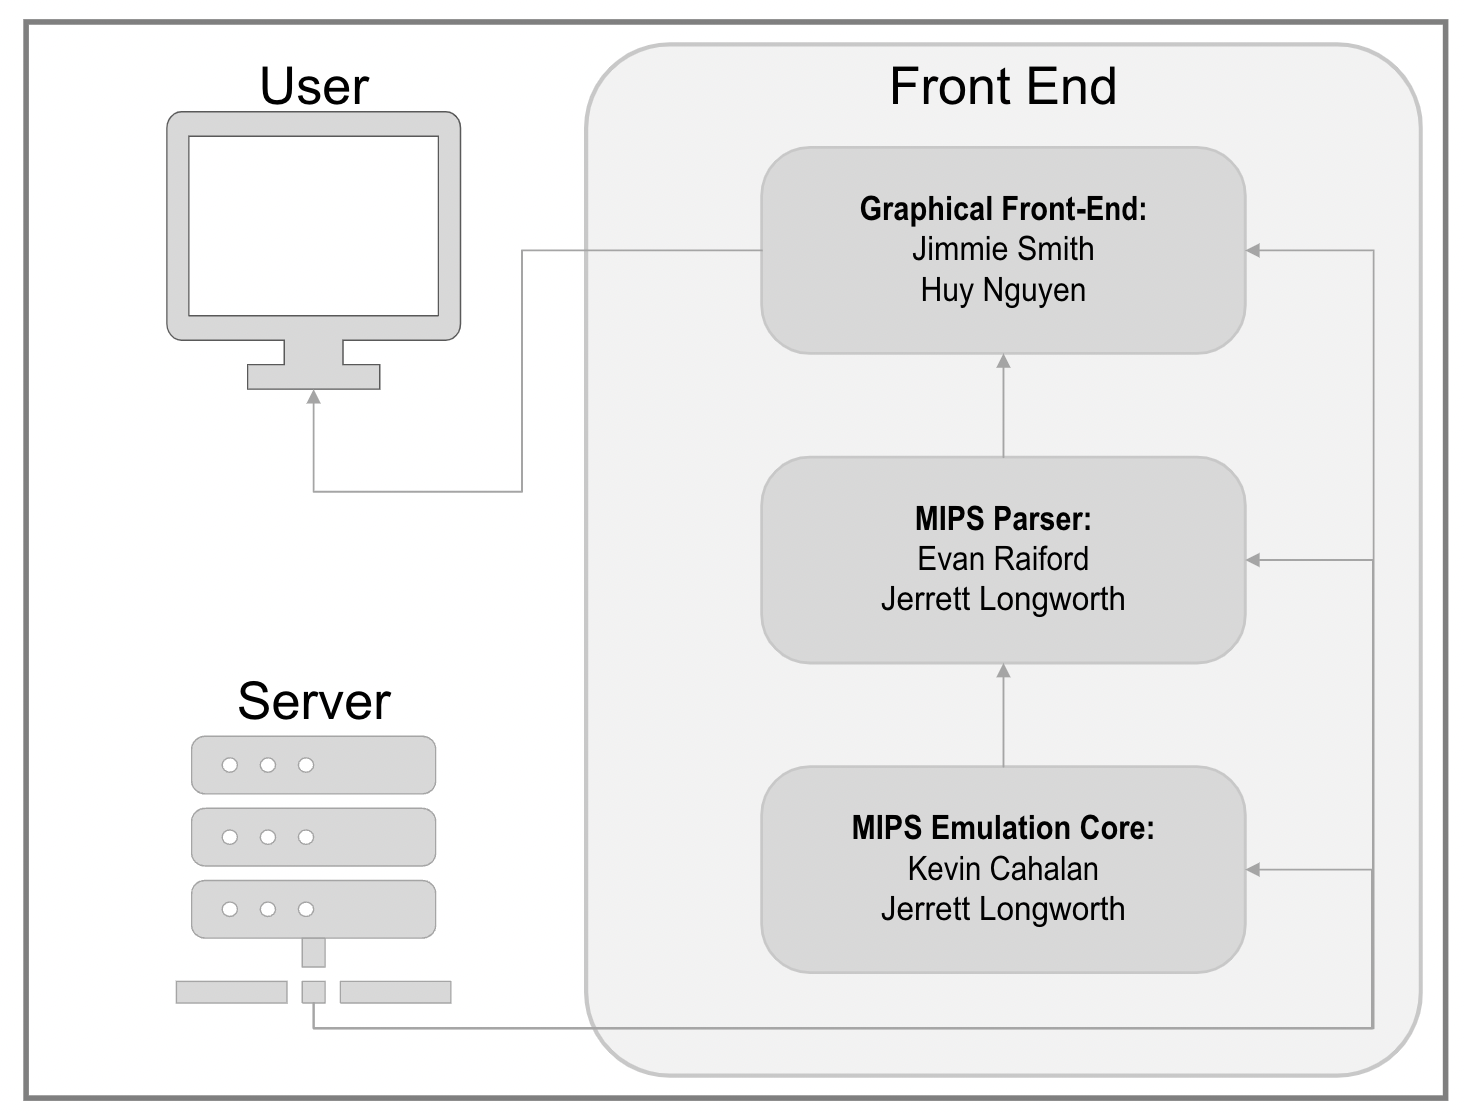
\includegraphics[width=\textwidth]{block-diagram}
    \caption{Basic Block Diagram of OurSPIM}
\end{figure}



\section{Project Milestones (WIP)}
\begin{longtable}{| p{0.15\textwidth} | p{0.85\textwidth} |}
    \hline
    \textbf{Date} & \textbf{Milestone}\\\hline\hline
    09/19/2022 & Group introductions - Initial date to meet team members, discuss goals and ideas, and to schedule weekly meetings.\\\hline
    09/23 & First regularly-scheduled group meeting - Collaboration on project requirements, choice of language(s) and framework(s), and project roles.\newline \textbf{Note: Every future regularly-scheduled meeting may not be listed here.}\newline\newline Group members begin self-learning the language and frameworks planned to be used for this project (Docker, Rust, Yew). Collaboration on the initial design proposal begins.\\\hline
    09/27-10/04 & Get taken out for a week due to Hurricane Ian. :')\\\hline
    10/05 & TA check-in \#1. (Show 3-5 pages contributed per member)\\\hline
    10/07 & Regularly-scheduled group meeting - Final discussion, clarifications, and wrap-up of the Initial Design Proposal.\\\hline
    10/07 & Assignment 3 (Initial Design Proposal) is due. (15 pages total)\\\hline
    10/15 & The first major self-study milestone is for each member to get a basic web application up and running. Ideally, this starter application will be done in a way most similar to how we want the final product to be set up. This can be achieved by having each team member be familiar with Docker, Rust and other technologies needed.\\\hline
    10/19 & Meet with Dr. Gerber to check progress and understanding of the project.\\\hline
    10/21 & Regularly-scheduled group meeting - Project status and design document review.\\\hline
    10/31 & Assignment 4 (Individual pages in design document) is due. (15 pages per member contributed)\\\hline
    11/07 & TA check-in \#2. (Show 20-25 pages contributed per member)\\\hline
    11/18 & Emulation of basic MIPS instructions (such as add, sw, lw). This is where the debugger can be written as it will become handy down the line.\\\hline
    11/25 & A basic in-browser GUI is created. A space to enter MIPS assembly instructions in binary and some way to watch what the emulation core is doing.\\\hline
    12/07 & Final Design Document is due. (30 pages per member contributed)\\\hline
    12/11 & Fall 2022 / Senior Design 1 concludes.\newline \textbf{Note: There will be no milestones over the winter break, but group members will continue to work on the project with periodic meetings.}\\\hline
    01/09/2023 & Spring 2023 / Senior Design 2 begins. Resume scheduled group activity.\\\hline
    01/14 & More MIPS instructions are supported in the emulation core. MIPS64 support is introduced.\\\hline
    01/20 & In-browser parsing and assembling of MIPS assembly code. This could initially be done with libraries.\\\hline
    02/01 & All planned instructions from the MIPS64 ISA are supported by the emulation core.\\\hline
    02/15 & Full in-browser interface is functional.\\\hline
    03/01 & All high-priority features are completed. Polishing the GUI and frontend.\\\hline
    03/15 & Demo with Dr. Gerber/Dr. Leinecker.\\\hline
    04/17 & Final Design Document due and presentations.\\\hline
\end{longtable}



\section{Gantt Chart}
\begin{figure}[H]
    \centering
    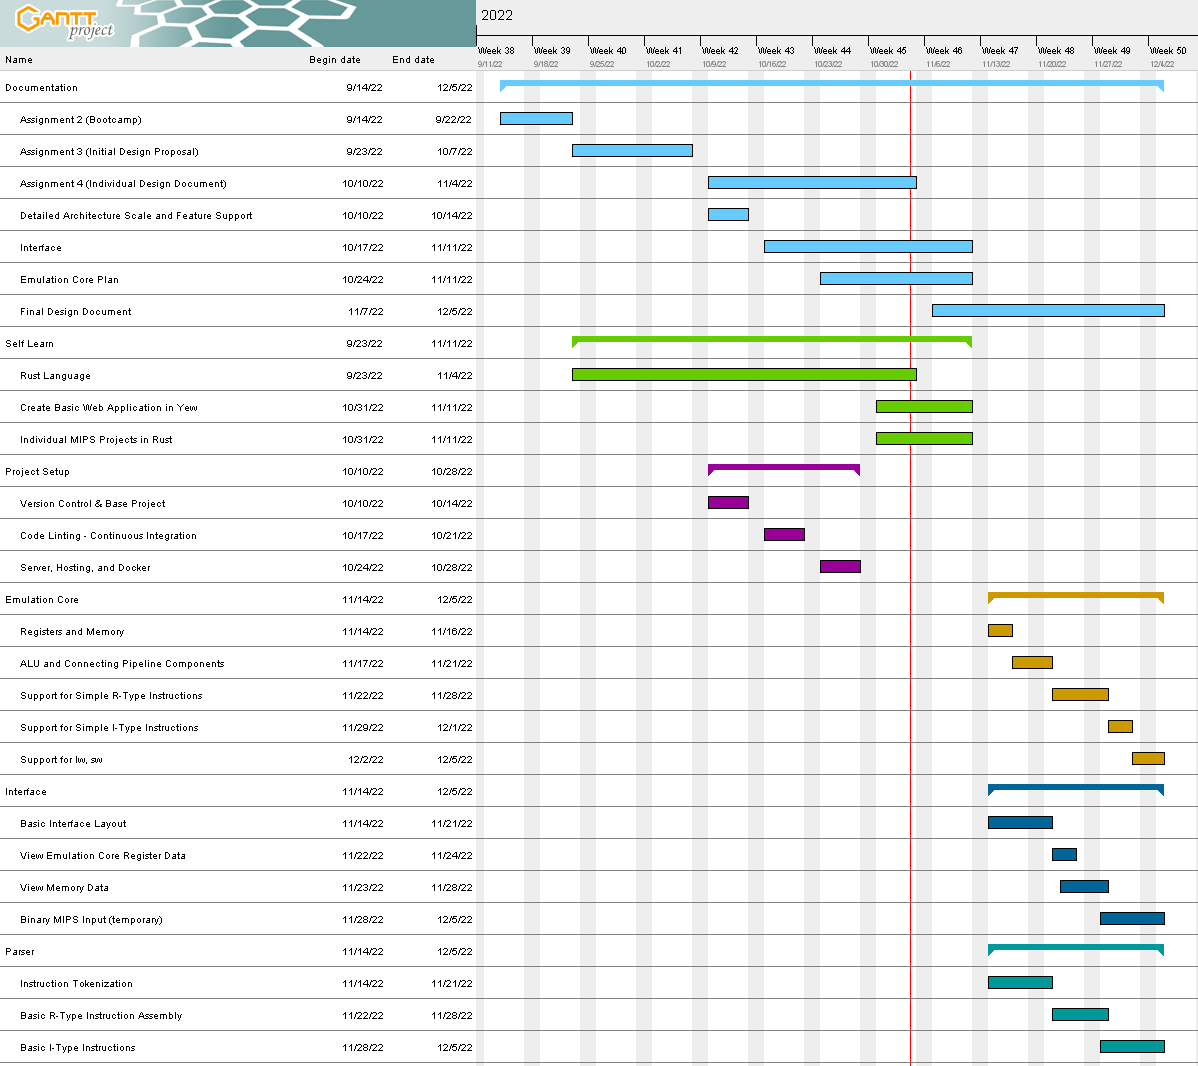
\includegraphics[width=\textwidth]{gantt-sd1}
    \caption{Senior Design 1 Gantt Chart}
\end{figure}

\begin{figure}[H]
    \centering
    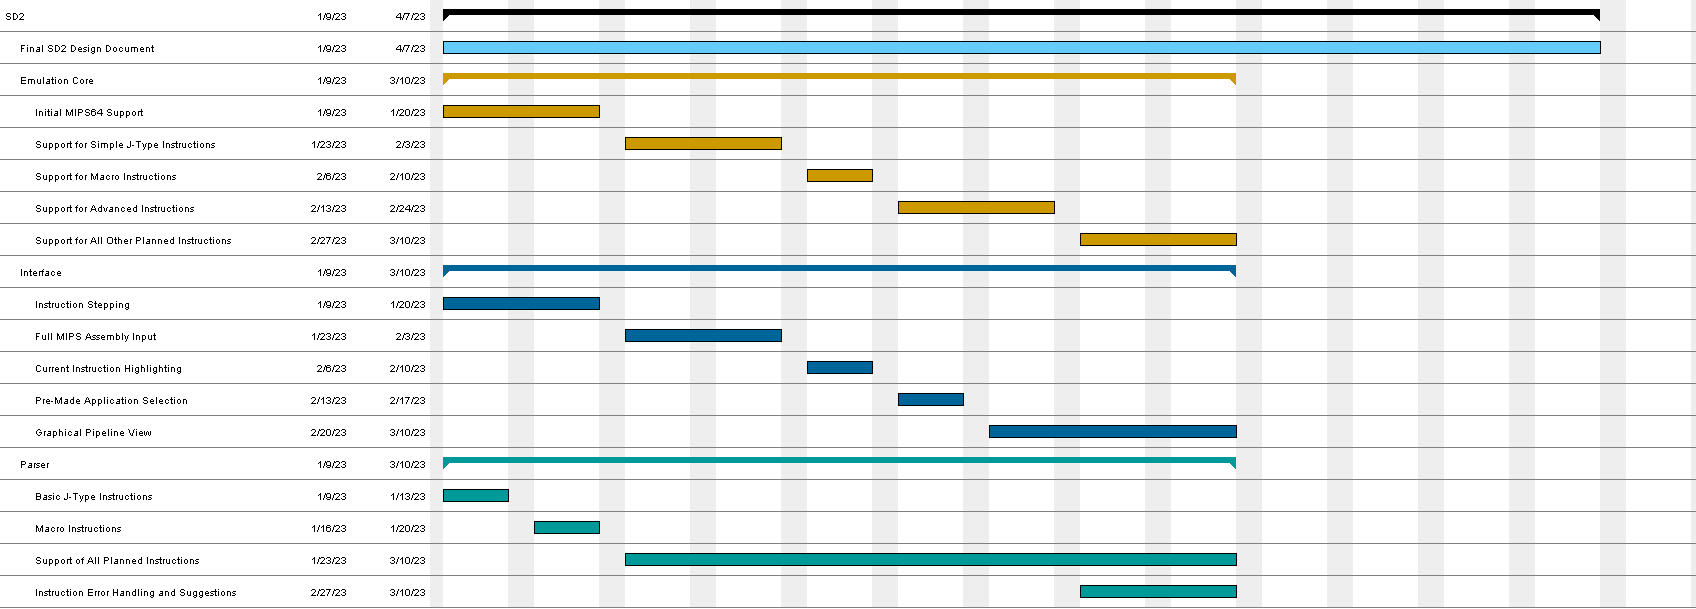
\includegraphics[width=\textwidth]{gantt-sd2}
    \caption{Senior Design 2 Gantt Chart}
\end{figure}
\clearpage



\bibliographystyle{ieeetr}
\bibliography{references} % Entries are in the references.bib file

\end{document}